\chapter{Aplikacja mobilna}
Aplikacja stworzona w ramach pracy pozwala na konfigurację oraz komunikację z wcześniej opisanym robotem minisumo. Z racji, iż została napisana w natywnym języku \textit{Swift} wspieranym systemem operacyjnym jest system iOS.

\section{Kompatybilność}
Jedynym wymogiem, który musi zostać spełniony w celu uruchomienia aplikacji jest wersja systemu – nie starsza niż \textit{iOS 10}. W związku z czym aplikacja z powodzeniem powinna działać zarówno na tabletach oraz telefonach marki \textit{Apple} posiadających wspomnianą lub nowszą wersję systemu. 

Docelowo aplikacja była uruchamiana oraz testowana na urządzeniu \textit{iPhone 5}, który jest najstarszym telefonem wspierającym system iOS 10. Powodem wyboru urządzenia była optymalizacja, a mianowicie poprawność działania aplikacji na najsłabszych podzespołach gwarantowała odpowiednią pracę na mocniejszych jednostkach.

Dodatkowo poprawność wyświetlania oraz skalowania została przetestowana w symulatorze dostarczonym wraz z środowiskiem \textit{Xcode} na urządzeniach takich jak \textit{iPhone 6 Plus} oraz \textit{iPad Pro}.
 
\section{Wzorzec MVC}
Aplikacja mobilna została zaprojektowana została według wzorca architektonicznego MVC (z~ang. \textit{Model–View–Controller}), który często wykorzystywany jest do tworzenia interfejsów użytkownika. W omawianym wzorcu można wyróżnić trzy obiekty:
\begin{itemize}
\item model – odpowiada za serwowanie danych,
\item widok – odpowiada za wizualizację danych, 
\item kontroler – reaguje na poczynania użytkownika, zarządza odświeżeniem widoków oraz aktualizacją modelu. 
\end{itemize}
Podział opisanych ról przedstawiono na rysunku ~\ref{fig:mvc}.
\begin{figure}[H]
	\centering
		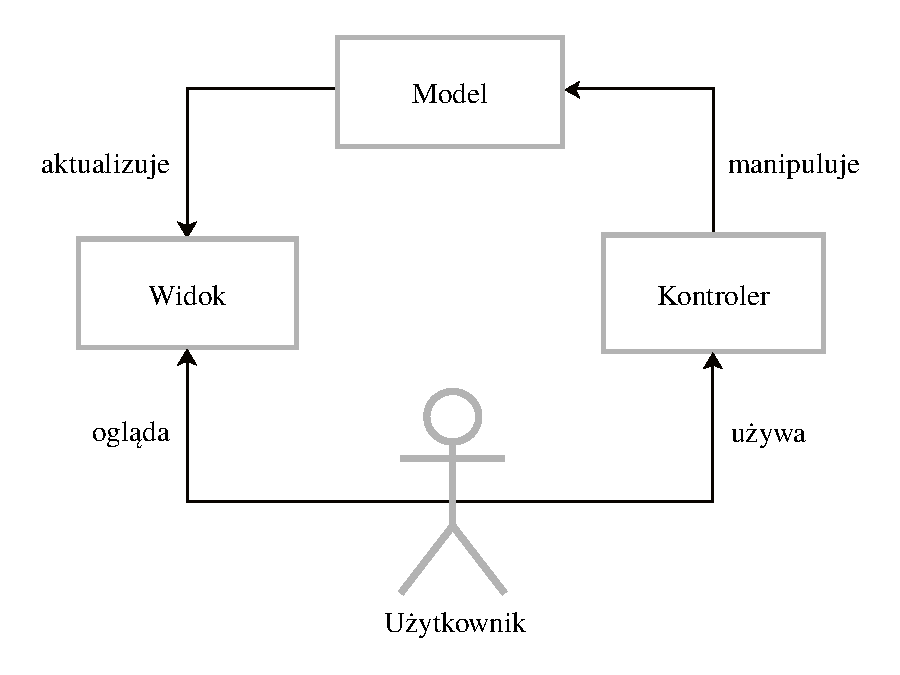
\includegraphics[width=0.75\linewidth]{pic05/mvc.pdf}
	\caption{Podział ról we wzorcu MVC.}
	\label{fig:mvc}	
\end{figure}

Dzięki wykorzystaniu tego wzorca uniezależniono przechowywane dane od sposobu w jaki są one przedstawiane użytkownikowi.

\section{Komunikacja}


\section{Struktura aplikacji}
Tak jak wcześniej wspomniano, aplikacja została stworzona przy użyciu wzorca \textit{MVC}. Poniżej przedstawiono strukturę plików aplikacji.

\begin{figure}[H]
	\centering
		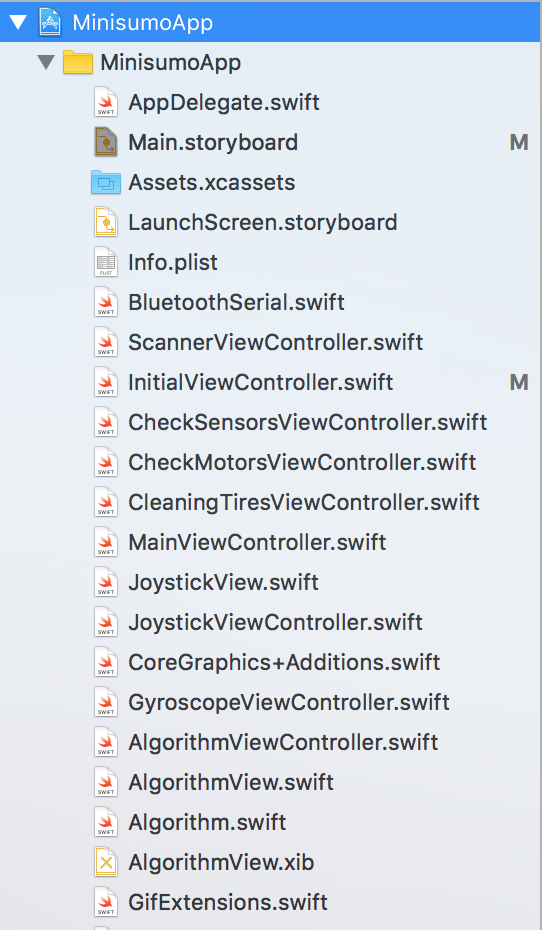
\includegraphics[width=0.75\linewidth, height=10cm, keepaspectratio]{pic05/structure.png}
	\caption{Struktura plików aplikacji mobilnej.}
	\label{fig:structure}	
\end{figure}

Na rysunku \ref{fig:structure} pliki o rozszerzeniu \textit{swift}, których nazwy kończą się na \textit{Controller} pełnią rolę kontrolerów, a \textit{View} widoków przedstawianych użytkownikowi. Reszta plików odpowiedzialna jest za logikę aplikacji. Dodatkowo plik \textit{Main.storyboard} zawiera konfiguracje większości widoków stworzonych przy użyciu graficznego narzędzia dostarczonego przez środowisko \textit{Xcode}.

\subsection{Widok główny}
\subsection{Widok sterowania automatycznego}
\subsection{Widok sterowania zdalnego}
\subsection{Widok diagnostyki}